\documentclass{article}
\usepackage[romanian]{babel}
\usepackage{geometry}
\usepackage{amsmath}
\usepackage{graphicx}
\usepackage{tcolorbox}
\usepackage{tikz}
\usepackage{pgfplots}
\usepackage{hyperref}
\usepackage{amssymb} 
\usepackage{pifont}  
\usepackage{enumitem} 
\usepackage{amsmath}
\usepackage{amssymb}
\usetikzlibrary{shapes, arrows.meta, positioning}

\title{Învățare automată - Temă S10}
\author{Balan Călin (3B1)}
\date{6 decembrie 2024}
\begin{document}
\maketitle

\section*{Problema 0.164A / pag. 254}

Cunoaștem \( f \) funcție derivabilă, \( f : \mathbb{R}^d \to \mathbb{R} \). \newline
Regula de actualizare este: \( x_i^{(k+1)} \leftarrow x_i^{(k)} - learningRate \cdot \frac{\partial}{\partial x_i} f(x^{(k)}) \)

\noindent \textbf{a}.

\( f(x) = 4x^2 - 2x + 1 \)

\( learningRate = 0.1 \)

\(\frac{\partial}{\partial x}f(x) = \frac{\partial}{\partial x}(4x^2-2x+1) = 8x-2\)

\( x^{(1)} = 1 \)

Pentru \( k = 0 \):

\( \frac{\partial}{\partial x} f(x^{(0)}) = 6 \)

\( x^{(1)} = x^{(0)} - learningRate \cdot 6 = 1 - 0.1 \cdot 6 = 0.4 \)

\( f(x^{(1)}) = f(0.4) = 0.84 \)

Pentru \( k = 1 \):

\( \frac{\partial}{\partial x} f(x^{(1)}) = 1.2 \)

\( x^{(2)} = x^{(1)} - learningRate \cdot 1.2 = 0.4 - 0.1 \cdot 1.2 = 0.28 \)

\( f(x^{(2)}) = f(0.28) = 0.7536 \)

Pentru \( k = 2 \):

\( \frac{\partial}{\partial x} f(x^{(2)}) = 0.24 \)

\( x^{(3)} = x^{(2)} - learningRate \cdot 0.24 = 0.28 - 0.1 \cdot 0.24 = 0.256 \)

\( f(x^{(3)}) = f(0.256) = 0.7501 \)

\noindent \textbf{b}.

\( f(x_1, x_2) = x_1^2 + sin(x_1 + x_2) + x_2^2 \)

\( x^{(k)} = (x_1^{(k)}, x_2^{(k)}) \)

\( x_1^{(k+1)} \leftarrow x_1^{(k)} - learningRate \cdot \frac{\partial}{\partial x_1} f(x_1^{(k)}, x_2^{(k)}) \)

\( x_2^{(k+1)} \leftarrow x_2^{(k)} - learningRate \cdot \frac{\partial}{\partial x_2} f(x_1^{(k)}, x_2^{(k)}) \)

\( \frac{\partial}{\partial x_1} f(x_1^{(k)}, x_2^{(k)}) = 2x_1 + cos(x_1 + x_2) \)

\( \frac{\partial}{\partial x_2} f(x_1^{(k)}, x_2^{(k)}) = 2x_2 + cos(x_1 + x_2) \)

\( f : [-4, 4] \to [-4, 4] \)

\textbf{i}. Primii 10 pași făcuți de \textbf{GD} începând cu \( (x_1^{(0)}, x_2^{(0)}) = (3, -3) \) și \( learningRate = 0.4 \):

\begin{center}
    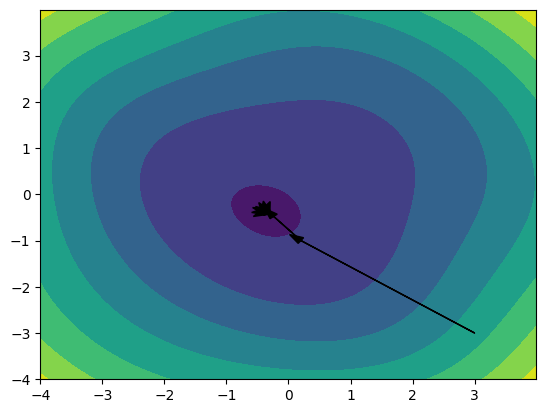
\includegraphics[width=0.5\textwidth]{1.png}
\end{center}

\textbf{ii}. Primii 10 pași făcuți de \textbf{GD} începând cu \( (x_1^{(0)}, x_2^{(0)}) = (3, -3) \) și \( learningRate = 0.8 \):

\begin{center}
    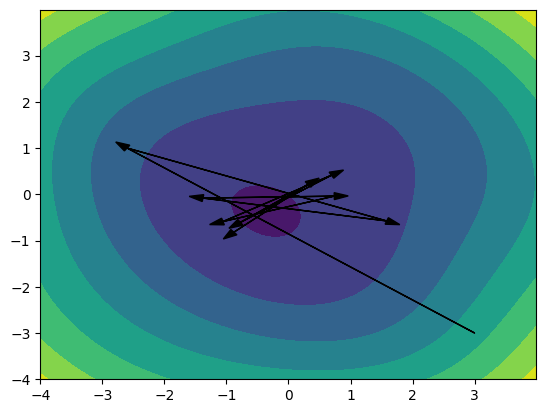
\includegraphics[width=0.5\textwidth]{2.png}
\end{center}

Se observă faptul că punctele converg către o valoare de minim. Mai mult, \( learningRate \)-ul configurează dimensiunea "pașilor" cu care covergența are loc.

\section*{Problema 1.34 / pag. 332}

Vom schimba setul de date inițial cu cel de la \textbf{Problema 4.6 / pag. 491}.

\noindent Astfel, vom face următoarele translări pentru a ne ajuta în rezolvarea problemei curent:
\begin{itemize}
    \item Clasa: \( X_1 \in \{0, 1\} \), unde I = 0, Inferioară = 1;
    \item Sexul: \( X_2 \in \{0, 1\} \), unde Masculin = 0, Feminin = 1;
    \item Vârsta: \( X_3 \in \{0, 1\} \), unde Copil = 0, Adult = 1;
    \item Supraviețuitor: \( Y \in \{0, 1\} \), unde Nu = 0, Da = 1.
\end{itemize}

Setul de date devine:

\begin{tabular}{|c|c|c|c|c|c|}
    \hline
    Indecși & Număr & \( X_1 \) & \( X_2 \) & \( X_3 \) & \( Y \) \\ \hline
    \( [1, 5] \) & \( 5 \) & \( 0 \) & \( 0 \) & \( 0 \) & \( 1 \) \\ \hline
    \( [6, 123] \) & \( 118 \) & \( 0 \) & \( 0 \) & \( 1 \) & \( 0 \) \\ \hline
    \( [124, 180] \) & \( 57 \) & \( 0 \) & \( 0 \) & \( 1 \) & \( 1 \) \\ \hline
    \( [181, 181] \) & \( 1 \) & \( 0 \) & \( 1 \) & \( 0 \) & \( 1 \) \\ \hline
    \( [182, 185] \) & \( 4 \) & \( 0 \) & \( 1 \) & \( 1 \) & \( 0 \) \\ \hline
    \( [186, 325] \) & \( 140 \) & \( 0 \) & \( 1 \) & \( 1 \) & \( 1 \) \\ \hline
    \( [326, 360] \) & \( 35 \) & \( 1 \) & \( 0 \) & \( 0 \) & \( 0 \) \\ \hline
    \( [361, 384] \) & \( 24 \) & \( 1 \) & \( 0 \) & \( 0 \) & \( 1 \) \\ \hline
    \( [385, 1595] \) & \( 1211 \) & \( 1 \) & \( 0 \) & \( 1 \) & \( 0 \) \\ \hline
    \( [1596, 1876] \) & \( 281 \) & \( 1 \) & \( 0 \) & \( 1 \) & \( 1 \) \\ \hline
    \( [1877, 1893] \) & \( 17 \) & \( 1 \) & \( 1 \) & \( 0 \) & \( 0 \) \\ \hline
    \( [1894, 1920] \) & \( 27 \) & \( 1 \) & \( 1 \) & \( 0 \) & \( 1 \) \\ \hline
    \( [1921, 2025] \) & \( 105 \) & \( 1 \) & \( 1 \) & \( 1 \) & \( 0 \) \\ \hline
    \( [2026, 2201] \) & \( 176 \) & \( 1 \) & \( 1 \) & \( 1 \) & \( 1 \) \\ \hline
\end{tabular}

\noindent \textbf{a}.

\( l(w) = \sum_{i=1}^{2201} (y^{(i)} \ln \sigma (w \cdot x^{(i)}) + (1 - y^{(i)}) \ln (1 - \sigma (w \cdot x^{(i)})) ) 
= 5 \cdot 1 \cdot \ln \sigma (w \cdot (1, 0, 0, 0)^T) + 118 \cdot (1 - 0) \cdot \ln (1 - \sigma (w \cdot (1, 0, 0, 1)^T)) 
+ 57 \cdot 1 \cdot \ln \sigma (w \cdot (1, 0, 0, 1)^T) + 1 \cdot 1 \cdot \ln \sigma (w \cdot (1, 0, 1, 0)^T) 
+ 4 \cdot (1 - 0) \cdot \ln (1 - \sigma (w \cdot (1, 0, 1, 1)^T)) + 140 \cdot 1 \cdot \ln \sigma (w \cdot (1, 0, 1, 1)^T) 
+ 35 \cdot (1-0) \cdot \ln (1 - \sigma (w \cdot (1, 1, 0, 0)^T)) + 24 \cdot 1 \cdot \ln \sigma (w \cdot (1, 1, 0, 0)^T)
+ 1211 \cdot (1 - 0) \cdot \ln (1 - \sigma (w \cdot (1, 1, 0, 1)^T)) + 281 \cdot 1 \cdot \ln \sigma (w \cdot (1, 1, 0, 1)^T) 
+ 17 \cdot (1 - 0) \cdot \ln (1 - \sigma (w \cdot (1, 1, 1, 0)^T)) + 27 \cdot 1 \cdot \ln \sigma (w \cdot (1, 1, 1, 0)^T) 
+ 105 \cdot (1 - 0) \cdot \ln (1 - \sigma (w \cdot (1, 1, 1, 1)^T)) + 176 \cdot 1 \cdot \ln \sigma (w \cdot (1, 1, 1, 1)^T) 
= 5 \ln \sigma (w_0) + 118 \ln (1 - \sigma(w_0 + w_3)) + 57 \ln \sigma (w_0 + w_3) + \ln \sigma (w_0 + w_2) 
+ 4 \ln (1 - \sigma (w_0 + w_2 + w_3)) + 140 \ln \sigma (w_0 + w_2 + w_3) + 35 \ln (1 - \sigma (w_0 + w_1)) + 24 \ln \sigma (w_0 + w_1) 
+ 1211 \ln (1 - \sigma (w_0 + w_1 + w_3)) + 281 \ln \sigma (w_0 + w_1 + w_3) + 17 \ln (1 - \sigma (w_0 + w_1 + w_2)) + 27 \ln \sigma (w_0 + w_1 + w_2) 
+ 105 \ln (1 - \sigma (w_0 + w_1 + w_2 + w_3)) + 176 \ln \sigma (w_0 + w_1 + w_2 + w_3) \)

\noindent \textbf{b}.

\textbf{i}.

\( \nabla_w l(w) = \sum_{i=1}^{2201} [ y^{(i)} - \sigma (w \cdot x^{(i)}) ] x^{(i)} 
= 5 [ 1 - \sigma (w_0) ] (1, 0, 0, 0)^T - 118 \sigma (w_0 + w_3) (1, 0, 0, 1)^T + 57 [ 1 - \sigma (w_0 + w_3) ] (1, 0, 0, 1)^T 
+ [ 1 - \sigma (w_0 + w_2) ] (1, 0, 1, 0)^T - 4 \sigma (w_0 + w_2 + w_3) (1, 0, 1, 1)^T + 140 [ 1 - \sigma (w_0 + w_2 + w_3) ] (1, 0, 1, 1)^T 
- 35 \sigma (w_0 + w_1) (1, 1, 0, 0)^T + 24 [ 1 - \sigma (w_0 + w_1) ] (1, 1, 0, 0)^T 
-1211 \sigma (w_0 + w_1 + w_3) (1, 1, 0, 1)^T + 281 [ 1 - \sigma (w_0 + w_1 + w_3) ] (1, 1, 0, 1)^T 
- 17 \sigma (w_0 + w_1 + w_2) (1, 1, 1, 0)^T + 27 [ 1 - \sigma (w_0 + w_1 + w_2) ] (1, 1, 1, 0)^T 
-105 \sigma (w_0 + w_1 + w_2 + w_3) (1, 1, 1, 1)^T + 176 [ 1 - \sigma (w_0 + w_1 + w_2 + w_3) ] (1, 1, 1, 1)^T 
= (711 - 5 \sigma (w_0) - 175 \sigma (w_0 + w_3) - \sigma (w_0 + w_2) - 144 \sigma (w_0 + w_2 + w_3) 
- 59 \sigma (w_0 + w_1) - 1492 \sigma (w_0 + w_1 + w_3) - 44 \sigma (w_0 + w_1 + w_2) - 281 \sigma (w_0 + w_1 + w_2 + w_3), 
508 - 59 \sigma (w_0 + w_1) - 1492 \sigma (w_0 + w_1 + w_3) - 44 \sigma (w_0 + w_1 + w_2) - 281 \sigma (w_0 + w_1 + w_2 + w_3),
344 - \sigma (w_0 + w_2) - 144 \sigma (w_0 + w_2 + w_3) - 44 \sigma (w_0 + w_1 + w_2) - 281 \sigma (w_0 + w_1 + w_2 + w_3), 
654 - 175 \sigma (w_0 + w_3) - 144 \sigma (w_0 + w_2 + w_3) - 1492 \sigma (w_0 + w_1 + w_3) - 281 \sigma (w_0 + w_1 + w_2 + w_3) )^T \)

\textbf{ii}.

Alegem \( j = 2 \):

\( \frac{\partial}{\partial w_2} l(w) = \frac{\partial}{\partial x_2} \ln \sigma (w_0 + w_2) 
+ \frac{\partial}{\partial x_2} 4 \ln (1 - \sigma (w_0 + w_2 + w_3)) + \frac{\partial}{\partial x_2} 140 \ln \sigma (w_0 + w_2 + w_3) 
+ \frac{\partial}{\partial x_2} 17 \ln (1 - \sigma (w_0 + w_1 + w_2)) + \frac{\partial}{\partial x_2} 27 \ln \sigma (w_0 + w_1 + w_2) 
+ \frac{\partial}{\partial x_2} 105 \ln (1 - \sigma (w_0 + w_1 + w_2 + w_3)) + \frac{\partial}{\partial x_2} 176 \ln \sigma (w_0 + w_1 + w_2 + w_3) 
= 344 - \sigma (w_0 + w_2) - 144 \sigma (w_0 + w_2 + w_3) - 44 \sigma (w_0 + w_1 + w_2) -281 \sigma (w_0 + w_1 + w_2 + w_3) \)

Se poate ușor observa că rezultatul coincide cu poziția 2 din vectorul gradient calculat la \textbf{i}.

\noindent \textbf{c}.

\( w = 0 \in \mathbb{R}^4 \), deci \( w_i = 0, i \in \{0, 1, 2, 3\} \)

\( \sigma (z) = \frac{1}{1 + e^{-z}} \implies \sigma (0) = \frac{1}{1 + e^0} = 0.5 \)

\( \nabla_w l(w) = (711 - 5 \cdot 0.5 - 175 \cdot 0.5 - 0.5 - 144 \cdot 0.5 - 59 \cdot 0.5 - 1492 \cdot 0.5 - 44 \cdot 0.5 - 281 \cdot 0.5, 
508 - 59 \cdot 0.5 - 1492 \cdot 0.5 - 44 \cdot 0.5 -281 \cdot 0.5,
344 -0.5 - 144 \cdot 0.5 - 44 \cdot 0.5 - 281 \cdot 0.5,
654 - 175 \cdot 0.5 - 144 \cdot 0.5 - 1492 \cdot 0.5 - 281 \cdot 0.5 )^T 
= (-389.5, -430, 109, -392)^T \)

Aplicam rata de învățare: \( learningRate = 0.1 \)

\( 0.1 \cdot (-389.5, -430, 109, -392)^T = (-38.95, -43, 10.9, -39.2)^T \)

\noindent \textbf{d}.

Valorile optime pentru weight-uri sunt următoarele:

\( w = (0.3614, -1.1881, 2.1105, -0.6651) \)

Vom clasifica următoarele instanțe:

\begin{tabular}{|c|c|c|c|c|}
    \hline
    Nume & \( X_1 \) & \( X_2 \) & \( X_3 \) & \( Y \) \\ \hline
    U & \( 0 \) & \( 1 \) & \( 1 \) & \( ? \) \\ \hline
    V & \( 1 \) & \( 1 \) & \( 0 \) & \( ? \) \\ \hline
    W & \( 1 \) & \( 0 \) & \( 1 \) & \( ? \) \\ \hline
\end{tabular}

Clasificăm instanța U:

\( w_0 + w_1 \cdot x_1 + w_2 \cdot x_2 + w_3 \cdot x_3 
= 0.3614 + 0 \cdot -1.1881 + 1 \cdot 2.1105 + 1 \cdot -0.6651 
= 1.8068 > 0 \implies Y_U^{prediction} = 1 \)

Clasificăm instanța V:

\( w_0 + w_1 \cdot x_1 + w_2 \cdot x_2 + w_3 \cdot x_3 
= 0.3614 + 1 \cdot -1.1881 + 1 \cdot 2.1105 + 0 \cdot -0.6651 
= 1.2830 > 0 \implies Y_V^{prediction} = 1 \)

Clasificăm instanța W:

\( w_0 + w_1 \cdot x_1 + w_2 \cdot x_2 + w_3 \cdot x_3 
= 0.3614 + 1 \cdot -1.1881 + 0 \cdot 2.1105 + 1 \cdot -0.6651 
= -1.4918 < 0 \implies Y_W^{prediction} = 0 \)

\noindent \textbf{e}.

\textbf{i}.

\( H_w = - \sum_{i=1}^{n} h(x^{(i)}) (1 - h(x^{(i)})) x^{(i)} (x^{(i)})^T  \)

\( H_w = - \{ 5 \cdot \sigma (w_0) (1 - \sigma (w_0)) (1, 0, 0, 0)^T (1, 0, 0, 0) \\
+ 175 \cdot \sigma (w_0 + w_3) (1 - \sigma (w_0 + w_3)) (1, 0, 0, 1)^T (1, 0, 0, 1) \\
+ \sigma (w_0 + w_2) (1 - \sigma (w_0 + w_2)) (1, 0, 1, 0)^T (1, 0, 1, 0) \\
+ 144 \cdot \sigma (w_0 + w_2 + w_3) (1 - \sigma (w_0 + w_2 + w_3)) (1, 0, 1, 1)^T (1, 0, 1, 1) \\
+ 59 \cdot \sigma (w_0 + w_1) (1 - \sigma (w_0 + w_1)) (1, 1, 0, 0)^T Z(1, 1, 0, 0) \\
+ 1492 \cdot \sigma (w_0 + w_1 + w_3) (1 - \sigma (w_0 + w_1 + w_3)) (1, 1, 0, 1)^T (1, 1, 0, 1) \\
+ 44 \cdot \sigma (w_0 + w_1 + w_2) (1 - \sigma (w_0 + w_1 + w_2)) (1, 1, 1, 0)^T (1, 1, 1, 0) \\
+ 281 \cdot \sigma (w_0 + w_1 + w_2 + w_3) (1 - \sigma (w_0 + w_1 + w_2 + w_3)) (1, 1, 1, 1)^T (1, 1, 1, 1) \} \)

\textbf{ii}.

Alegem \( j = 2 \) și \( k = 1 \):

\( H_w (1, 2) = \frac{\partial^2}{\partial w_1 \partial w_2} l (w) 
= \frac{\partial}{\partial w_1} (\frac{\partial}{\partial w_2} l (w)) 
= \frac{\partial}{\partial w_1} ( 344 - \sigma (w_0 + w_2) - 144 \sigma (w_0 + w_2 + w_3) - 44 \sigma (w_0 + w_1 + w_2) - 281 \sigma (w_0 + w_1 + w_2 + w3) ) 
= -44 \sigma (w_0 + w_1 + w_2) \cdot (1 - \sigma (w_0 + w_1 + w_2)) - 281 \sigma (w_0 + w_1 + w_2 + w_3) \cdot (1 - \sigma (w_0 + w_1 + w_2 + w_3)) \)

Se poate vedea că rezultatul obținut coincide cu cel de pe linia și coloana corespunzătoare din hessiană.

\textbf{iii}.

Vom calcula \( H(2, 1) \) și verifica egalitatea cu \( H(1, 2) \).

\( H(2, 1) = \frac{\partial^2}{\partial w_2 \partial w_1} l(w) = \frac{\partial}{\partial w_2} (\frac{\partial}{\partial w_1} l(w)) 
= \frac{\partial}{\partial w_2} ( 35 \ln (1 - \sigma (w_0 + w_1)) + 24 \ln \sigma (w_0 + w_1) + 1211 \ln (1 - \sigma (w_0 + w_1 + w_3)) 
+ 281 \ln \sigma (w_0 + w_1 + w_3) + 17 \ln (1 - \sigma (w_0 + w_1 + w_2)) + 27 \ln \sigma (w_0 + w_1 + w_2) 
+ 105 \ln (1 - \sigma (w_0 + w_1 + w_2 + w_3)) + 176 \ln \sigma (w_0 + w_1 + w_2 + w_3) ) 
= \frac{\partial}{\partial w_2} (508 - 59 \sigma (w_0 + w_1) - 1492 \sigma (w_0 + w_1 + w_3) - 44 \sigma (w_0 + w_1 + w_2) - 281 \sigma (w_0 + w_1 + w_2 + w_3)) 
= -44 \sigma (w_0 + w_1 + w_2) (1 - \sigma (w_0 + w_1 + w_2)) - 281 \sigma (w_0 + w_1 + w_2 + w_3) (1 - \sigma (w_0 + w_1 + w_2 + w_3)) \)

Asadar, egalitatea cerută se respectă.

\noindent \textbf{f}.

Valorile optime obținute pentru \( w \) sunt următoarele:

\( w = (0.5231, -1.1903, 2.1018, -0.6594) \)

Modelul astfel obținut va clasifica identic instanțele de test, întrucât weight-urile converg către aceleași puncte.

Metoda gradientului necesita un număr de iterații semnificativ mai mare decât Newton-Raphson, întrucât cel din urma converge cu rată de ordin pătratic.
În schimb, timpul de execuție este mult mai mic in cazul metodei gradientului, deoarece Newton-Raphson necesită calcularea matricii hessiene.

\noindent \textbf{g}.

\( J(w) = \frac{1}{n} \sum_{i=1}^{n} \ln (1 + exp(-y^{'(i)} \cdot w \cdot x^{(i)})) 
= \frac{1}{2201} (5 \ln (1 + exp(-w_0)) + 118 \ln (1 + exp(w_0 + w_3)) + 57 \ln (1 + exp(-w_0 - w_3)) + \ln (1 + exp(-w_0 - w_2)) 
+ 4 \ln (1 + exp(w_0 + w_2 + w_3)) + 140 \ln (1+ exp(-w_0 - w_2 - w_3)) + 35 \ln (1 + exp (w_0 + w_1)) + 24 \ln (1 + exp(-w_0 - w_1)) 
+ 1211 \ln (1 + exp(w_0 + w_1 + w_3)) + 281 \ln (1 + exp(-w_0 - w_1 - w_2)) + 
105 \ln (1 + exp(w_0 + w_1 + w_2 + w_3)) + 176 \ln (1 + exp(-w_0 - w_1 - w_2 - w_3))) \)

Știm că \( 1 - \sigma (z) = \sigma (-z) \), unde \( z = w \cdot x \).

\( \sum_{i=1}^{n} \ln (1 + exp(-y^{(i)} \cdot w \cdot x^{(i)})) = \ln \prod_{i=1}^{n} (1 + exp(-y^{(i)} \cdot w \cdot x^{(i)})) \)

\( 1 + exp(-y^{(i)} \cdot w \cdot x^{(i)}) = \begin{cases}
1 + e^{-w \cdot x^{(i)}} = (\frac{1}{1 + e^{-w \cdot x^{(i)}}})^{-1} = (\sigma (w \cdot x^{(i)}))^{(-1)y^{'(i)}}, & \text{dacă } y^{'(i)} = 1, \\
1 + e^{w \cdot x^{(i)}} = (\frac{1}{1 + e^{w \cdot x^{(i)}}})^{-1} = (\sigma (-w \cdot x^{(i)}))^{(-1)y^{'(i)}}, & \text{dacă } y^{'(i)} = 0.
\end{cases} \)

Deci, pentru fiecare \( y^{(i)} \):

\( \ln (1 + exp(-y^{(i)} \cdot w \cdot x^{(i)})) = \begin{cases}
-\ln \sigma (w \cdot x^{(i)}), & \text{dacă } y^{(i)} = 1, \\
-\ln (1 - \sigma (w \cdot x^{(i)})), & \text{dacă } y^{(i)} = 0.
\end{cases} \)

Astfel, putem rescrie formula lui \( J(w) \), utilizând proprietățile logaritmului și definiția precendentă:

\( \ln \prod_{i=1}^{n} (\sigma (w \cdot x^{(i)}))^{-y^{(i)}} \cdot (1 - \sigma (w \cdot x^{(i)}))^{-(1-y^{(i)})} = -\sum_{i=1}^{n} (y^{(i)} \ln \sigma (w \cdot x^{(i)}) + (1 - y^{(i)}) \ln (1 - \sigma (w \cdot x^{(i)}))) \)

De unde reiese relația \( J(w) = -\frac{1}{n} l(w) \).

\end{document}